\documentclass{article}
\usepackage{caption}
\usepackage{hyperref}
\usepackage{subcaption}
% NeurIPS packages
\usepackage[preprint]{neurips_2023}  % Replace with [final] for the camera-ready version
\usepackage{graphicx}
\usepackage{amsmath}
\usepackage{amssymb}
% \usepackage{tikz}
% \usetikzlibrary{bayesnet}
% \usepackage{authblk}
\bibliographystyle{plain}

% Title
\title{Learning Bayesian Networks From Data}

\author{Pratik Karmakar\\
School of Computing,\\
National University of Singapore\\
CNRS@CREATE Ltd, Singapore\\
\texttt{pratik.karmakar@u.nus.edu}\\
\And
C\'eline Liu\\
School of Computing,\\
National University of Singapore\\
T\'el\'ecom Paris\\
\texttt{celine.liu@telecom-paris.fr}\\
\And
Nicholas Tan Yu Da\\
School of Computing,\\
National University of Singapore\\
\texttt{e0726708@u.nus.edu}}

% \author{
%   Pratik Karmakar\\National University of Singapore\\ CNRS@CREATE Ltd, 1 Create Way, Singapore \\
%  % ,  #08-01 CREATE Tower, Singapore 138602\\
%   \texttt{pratik.karmakar@u.nus.edu}
%   \and
%   C\'eline Liu\\T\'el\'ecom Paris\\National University of Singapore\\
%   \texttt{celine.liu@telecom-paris.fr}
%   \and
%   Nicholas Tan Yu Da\\National University of Singapore\\
%   \texttt{e0726708@u.nus.edu}
%   }

\begin{document}

% Make the title
\maketitle

% Abstract section
\begin{abstract}
\end{abstract}
% Sections
\section{Introduction}
We provide the experiments and necessary codes to reproduce our results in the github repository: \url{https://github.com/pratik2358/bayes_net_learning}
\section{Related Works}
\paragraph*{What to write}
\begin{itemize}
    \item Where did it start and how? - 2-3 sentences along with necessary references.
    \item Once Bayes net was introduced, what were the initial challenges? Cite proper works.
    \item How have researchers addressed the challenges? Cite proper works.
    \item If there exists no proper solution to some of the challenges yet, why? Cite proper works.
\end{itemize}

\paragraph*{Example citation}
The survey papers by Kitson et al.~\cite{kitson2023survey} and Scanagatta et al.~\cite{scanagatta2019survey} are our starting points.
% \section{Related Works}
Bayesian Network (BN) structure learning has been a significant topic in machine learning and artificial intelligence since its early introduction by Pearl~\cite{pearl1985bayesian} and others in the mid-1980s, where BNs were proposed as a framework for evidential reasoning and memory modeling . Over the years, substantial advancements have been made in both the theoretical underpinnings and practical implementations of BN learning algorithms.

Research on BN structure learning with continuous variables extended the initial focus on discrete variables, laying the groundwork for handling real-world applications where both types of variables are present. Moreover, methods to find the optimal BN structures, such as Perrier et al.'s~\cite{perrier2008finding} approach of utilizing a super-structure , advanced the ability to handle more complex networks efficiently.

Chickering's algorithm~\cite{silander2012simple} offered a simple but effective approach for finding globally optimal BN structures, marking a milestone in scalable algorithms . Complementing this, Peters et al.~\cite{peters2015structural} introduced the concept of structural intervention distance (SID), a metric for evaluating causal graphs by measuring differences between them, offering an innovative way to assess learned structures .

With the rise of high-dimensional data, algorithms such as the Fast Greedy Equivalence Search (FGES) were developed to handle massive datasets like fMRI, scaling BN learning to millions of variables . Meanwhile, the BDeu scoring function has seen rigorous theoretical analysis to understand its behavior and limitations in structure learning .

Several improvements in structure learning algorithms have been suggested to enhance both accuracy and scalability. Ramsey et al.~\cite{ramsey2016improving} presented an improved PC algorithm that enhances performance by maximizing p-values during structure search . The accuracy and efficiency of these algorithms were further benchmarked by studies comparing public causal search packages and advancing greedy search methods .

More recent surveys~\cite{scanagatta2019survey, kitson2023survey} have provided comprehensive overviews of state-of-the-art algorithms in BN structure learning, analyzing performance trade-offs in terms of speed, scalability, and structural accuracy. These surveys emphasize the need for balancing computational efficiency with the quality of learned networks, particularly as datasets grow larger and more complex.

This body of work highlights the evolution of BN structure learning algorithms and motivates our investigation into how data quantity affects structure learning performance across different algorithms, providing insights into both theoretical and practical improvements.
\section{Background}
\section{Methodology}

\section{Experiments}
\begin{figure}[htp!]
    \centering
    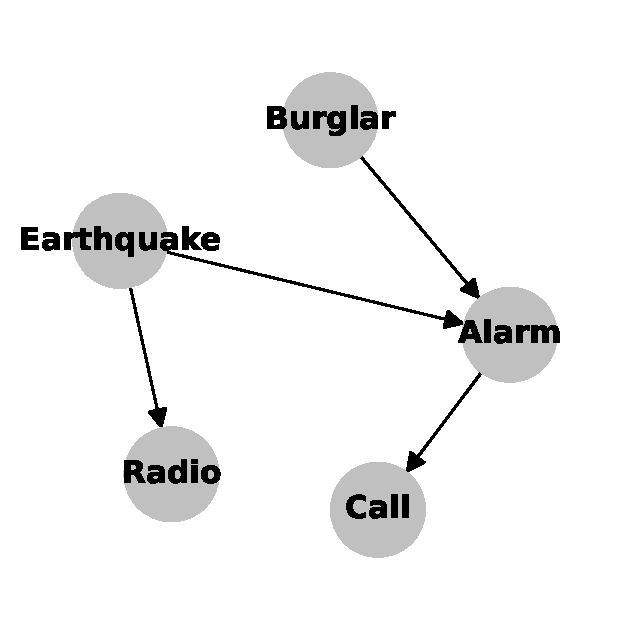
\includegraphics[width=0.5\linewidth]{plots/alarm.pdf}
    \caption{An example of a Bayesian Network to learn}
    \label{fig:alarm_fig}
\end{figure}
\begin{figure}[htp!]
     \centering
     \begin{subfigure}{0.7\textwidth}
         \centering
    
\includegraphics[width=\textwidth]{plots/legends.pdf}
     \end{subfigure}
     \begin{subfigure}{0.32\textwidth}
         \centering
         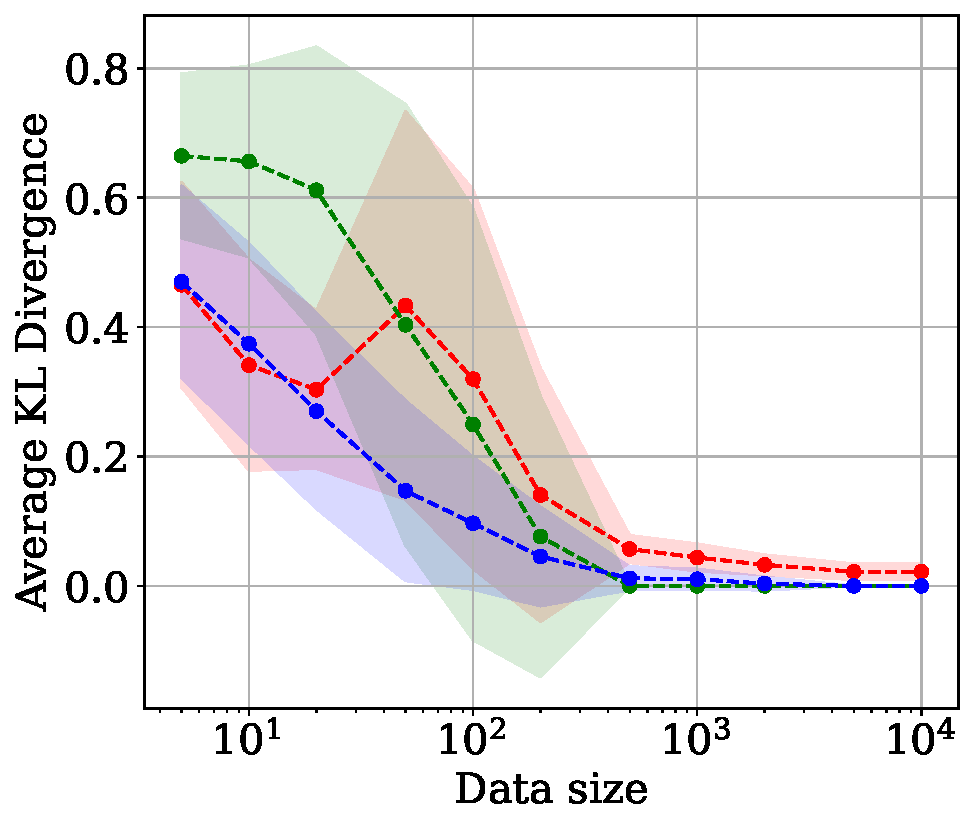
\includegraphics[width=\textwidth]{plots/kl_divergence.pdf}
         \caption{KL divergence between the probability distributions learned by the model and that observed in the data.}
         \label{fig:kl_div_dist}
     \end{subfigure}
     \hfill
     \begin{subfigure}{0.32\textwidth}
         \centering
         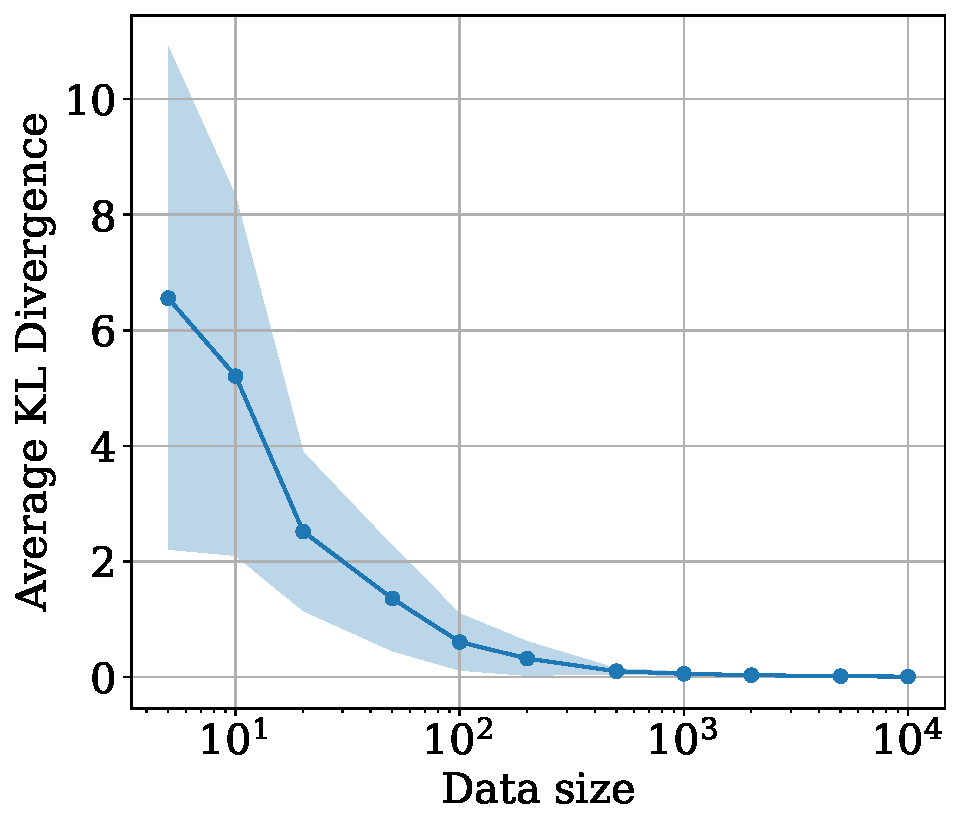
\includegraphics[width=\textwidth]{plots/joint_dist_div.pdf}
         \caption{KL divergence between the joint distributions observed from the samples from the model and that observed in the data.}
         \label{fig:kl_div_joint}
     \end{subfigure}
     \hfill
     \begin{subfigure}{0.32\textwidth}
         \centering
         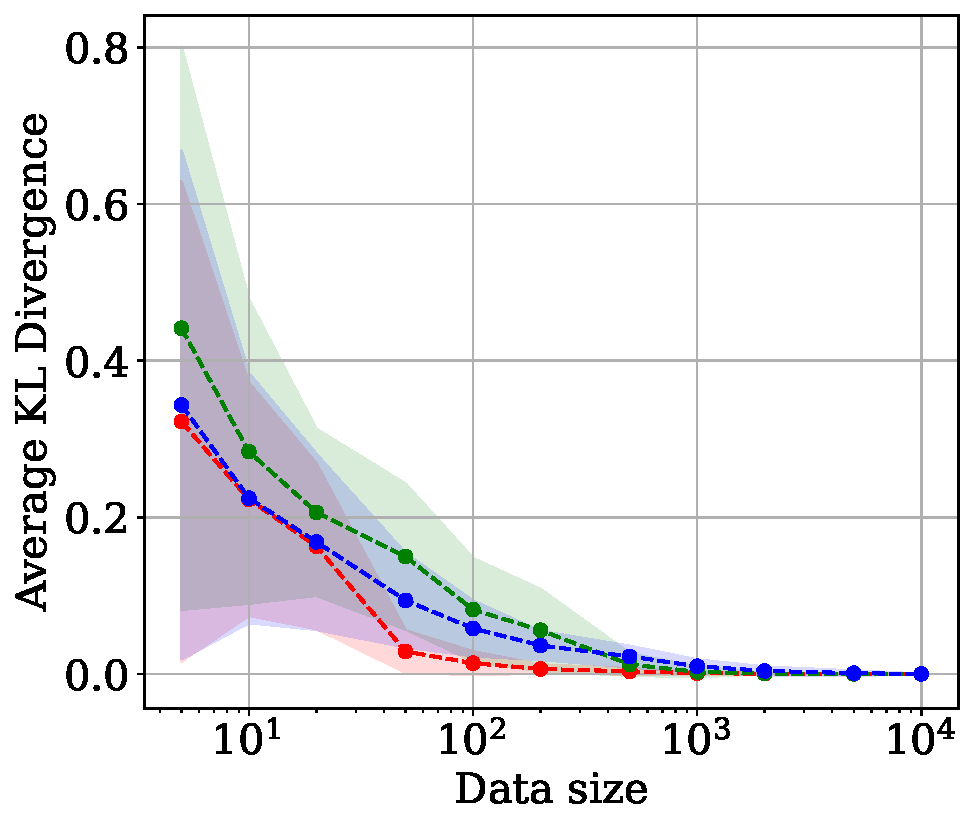
\includegraphics[width=\textwidth]{plots/conditionals_kl_divergence.pdf}
         \caption{KL divergence between the conditional distributions observed from the samples from the model and that observed in the data.}
         \label{fig:kl_div_marginals}
     \end{subfigure}
        \caption{Comparison among Exact algorithm (unbounded number of parents and 2 maximum parents) and Chow-Liu approximation algorithm for learning Bayesian networks from discrete data.}
        \label{fig:str_learning_comp}
\end{figure}

\begin{figure}[htp!]
\begin{subfigure}{0.7\textwidth}
         \centering
    
\includegraphics[width=\textwidth]{plots/legends.pdf}
     \end{subfigure}
    \centering
    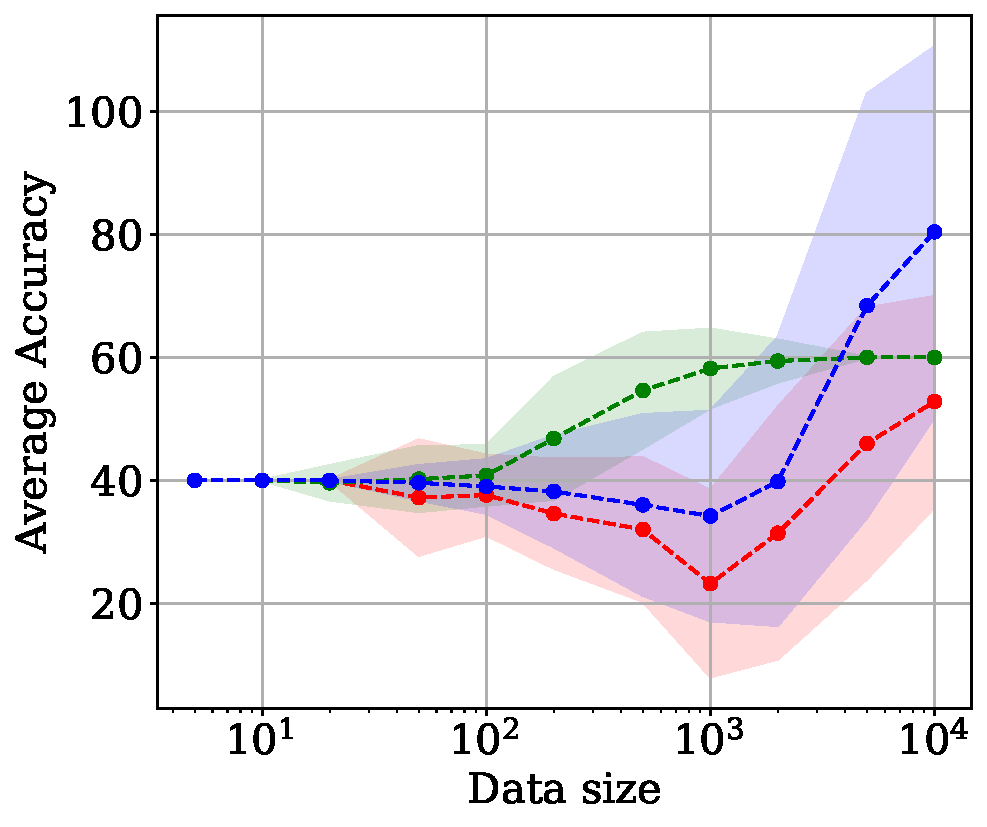
\includegraphics[width=0.5\linewidth]{plots/accuracy.pdf}
    \caption{Comparison of structural accuracy using Exact algorithm (unbounded number of parents and 2 maximum parents) and Chow-Liu approximation learning}
    \label{fig:str_acc}
\end{figure}
\section{Conclusion}

% References
\newpage
\bibliography{ref}

\end{document}
